\documentclass[11pt,a4paper]{article}
% Preamble for chain-load-balance paper
\usepackage[T1]{fontenc}
\usepackage[utf8]{inputenc}
\usepackage{lmodern}
\usepackage[margin=1in]{geometry}
\usepackage{microtype}
\usepackage{amsmath,amssymb,amsthm,mathtools}
\usepackage{booktabs}
\usepackage{enumitem}
\usepackage{hyperref}
\usepackage{tikz}
\usetikzlibrary{arrows.meta,positioning,fit,calc,backgrounds,decorations.pathreplacing}

\setlist[itemize]{leftmargin=1.5em}
\setlist[enumerate]{leftmargin=1.7em}

\newtheorem{definition}{Definition}
\newtheorem{remark}{Remark}
\newtheorem{proposition}{Proposition}

\newcommand{\Zone}{\mathcal{Z}}
\newcommand{\Loc}{\mathcal{L}}
\newcommand{\Ints}{\mathcal{I}}
\newcommand{\Chain}{\mathcal{C}}
\newcommand{\Front}{\mathcal{F}}
\newcommand{\Pend}{\mathcal{P}}
\newcommand{\Live}{\mathcal{A}}
\newcommand{\cost}{\mathrm{cost}}


\title{Chain-Level Load Imbalance in OpenMP Symbolic Reachability\\
A Formal Note with Practical Scheduling Directions}
\author{PTCTCL Design Note}
\date{\today}

\begin{document}
\maketitle

\begin{abstract}
This note formalizes why high thread counts in symbolic timed reachability do not imply proportional speedup.
We define zones, explain how per-discrete-state chains are created, and model chain settle cost under inclusion and convex-union rules.
Using this model, we derive starvation and tail-latency effects in level-synchronous OpenMP execution.
We then summarize algorithmic strategies used in related irregular-parallel systems and adapt them to this checker.
\end{abstract}

\section{Problem Statement}
In timed symbolic reachability, one explored item is not a cheap scalar state; it is a symbolic state with a dense DBM zone and non-trivial algebra.
Hence, with $T$ threads, one should not expect a throughput multiplier near $T$.

In the PTCTCL OpenMP path, successors are grouped by a discrete key $dk$ and processed in per-$dk$ chains.
These chains are irregular in size and computational cost.
At level barriers, a few heavy chains can dominate total level time while other workers idle.

The engineering question is therefore not ``how to use more threads'' but:
\begin{quote}
How to reduce chain-tail latency while preserving the exact symbolic semantics (subsumption + convex union behavior)?
\end{quote}

\section{Formal Model: Zones and Chains}
\subsection{Zone}
Let clocks be $x_1,\dots,x_n$ with reference clock $x_0=0$.
A zone is a convex set of valuations represented by a DBM:
\[
\Zone = \{\,\nu \in \mathbb{R}_{\ge 0}^n \mid \forall i,j:\ x_i - x_j \le c_{ij}\,\}.
\]
A symbolic state is
\[
s = (\ell, \iota, \Zone),
\]
where $\ell \in \Loc$ is a process-location vector and $\iota \in \Ints$ is an integer valuation.

\paragraph{Intuition.}
The DBM stores many concrete clock valuations at once.
So one ``state'' in this algorithm is already a compressed region of time-space, not one single point.
This is why per-state cost is high: each operation manipulates a whole polyhedral region encoded as a matrix.

\subsection{Discrete key and chain creation}
Define the discrete projection
\[
\pi(s) = dk = (\ell,\iota).
\]
All symbolic states with equal $dk$ are grouped into one chain:
\[
\Chain(dk) = \{\Zone_1,\Zone_2,\dots\}.
\]
Operationally, this is the per-key antichain container in the passed structure.

\paragraph{Intuition.}
Think of $dk$ as the ``control snapshot'' (which locations and integer values).
Inside that snapshot, time can still vary, so multiple zones are possible.
Those zones are exactly what form the chain.

\subsection{Settle operation per chain}
At one BFS level $L$, new zones for key $dk$ form pending set $\Pend_{dk}^{(L)}$.
Existing survivors are $\Live_{dk}^{(L-1)}$.
For each pending zone $z$, the checker applies:
\begin{enumerate}
  \item subsumed-by test: drop $z$ if $\exists a\in\Live: a\supseteq z$,
  \item reverse subsumption: remove $a$ if $z\supseteq a$,
  \item convex union attempts: if exact union succeeds, merge and continue.
\end{enumerate}
This induces dependence among updates inside the same chain.

\paragraph{Why dependence appears.}
If an early pending zone kills or merges a live zone, later pending zones are tested against a different survivor set.
So decisions are stateful within the same chain, which is exactly what limits trivial parallelization.

\begin{proposition}
Given order-sensitive convex union attempts, chain settle for one $dk$ is not trivially data-parallel without changing semantics.
\end{proposition}

\begin{proof}[Sketch]
Each accepted pending zone changes the future survivor set by killing/merging elements.
Subsequent decisions depend on this updated set, so naive parallel reordering can change outcomes.
\end{proof}

\subsection{Symbol glossary used in this note}
\begin{itemize}
  \item $\Zone$: one symbolic clock region (DBM zone).
  \item $dk$: discrete key $(\ell,\iota)$.
  \item $\Chain(dk)$: all zones stored for one discrete key.
  \item $\Pend_{dk}^{(L)}$: new zones for key $dk$ at BFS level $L$.
  \item $\Live_{dk}^{(L-1)}$: survivors already stored before settling level $L$.
\end{itemize}

\begin{figure}[t]
\centering
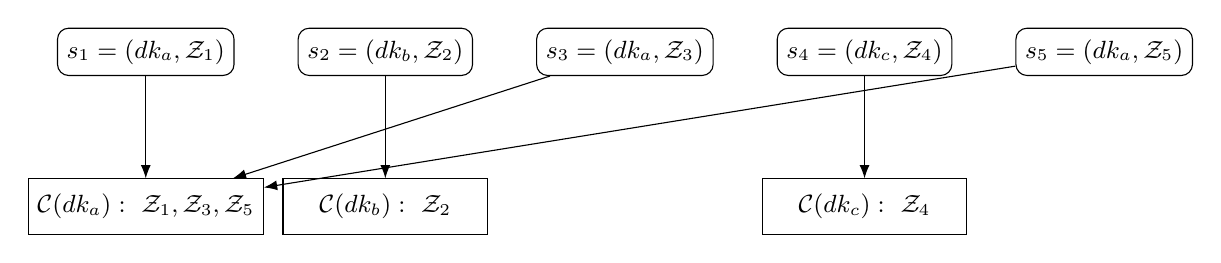
\begin{tikzpicture}[>=Latex, node distance=10mm]
  \tikzstyle{znode}=[draw, rounded corners, minimum width=18mm, minimum height=6mm, font=\small]
  \tikzstyle{cnode}=[draw, rectangle, minimum width=26mm, minimum height=7mm, font=\small]

  \node[znode] (s1) {$s_1=(dk_a,\Zone_1)$};
  \node[znode, right=8mm of s1] (s2) {$s_2=(dk_b,\Zone_2)$};
  \node[znode, right=8mm of s2] (s3) {$s_3=(dk_a,\Zone_3)$};
  \node[znode, right=8mm of s3] (s4) {$s_4=(dk_c,\Zone_4)$};
  \node[znode, right=8mm of s4] (s5) {$s_5=(dk_a,\Zone_5)$};

  \node[cnode, below=13mm of s1] (ca) {$\Chain(dk_a):\ \Zone_1,\Zone_3,\Zone_5$};
  \node[cnode, below=13mm of s2] (cb) {$\Chain(dk_b):\ \Zone_2$};
  \node[cnode, below=13mm of s4] (cc) {$\Chain(dk_c):\ \Zone_4$};

  \draw[->] (s1) -- (ca);
  \draw[->] (s3) -- (ca);
  \draw[->] (s5) -- (ca);
  \draw[->] (s2) -- (cb);
  \draw[->] (s4) -- (cc);
\end{tikzpicture}
\caption{Successors are projected by discrete key $dk$ into per-key chains.}
\label{fig:zone-to-chain}
\end{figure}


\section{Worked Example: How a Heavy Chain Emerges}
Suppose one frontier level emits successors whose discrete keys are:
\[
\underbrace{dk_a,dk_a,dk_a}_{3},\underbrace{dk_b,dk_b}_{2},\underbrace{dk_c,\dots,dk_c}_{40},\underbrace{dk_d}_{1},\underbrace{dk_e,\dots,dk_e}_{18}.
\]
Then pending counts are
\[
|\Pend_{dk_a}|=3,\ |\Pend_{dk_b}|=2,\ |\Pend_{dk_c}|=40,\ |\Pend_{dk_d}|=1,\ |\Pend_{dk_e}|=18.
\]
If prior live sizes are
\[
|\Live_{dk_a}|=2,\ |\Live_{dk_b}|=1,\ |\Live_{dk_c}|=55,\ |\Live_{dk_d}|=1,\ |\Live_{dk_e}|=12,
\]
a useful first-order cost proxy is
\[
\cost(dk) = \alpha\,|\Pend_{dk}|\,|\Live_{dk}| + \beta\,|\Pend_{dk}|^2.
\]
So
\[
\cost(dk_c) \gg \cost(dk_a),\cost(dk_b),\cost(dk_d),\cost(dk_e).
\]
Even with many threads, one worker processing $dk_c$ can dominate level completion.

\paragraph{How to read this example.}
Keys $dk_a,dk_b,\dots$ are not equally hard.
The chain for $dk_c$ is hard for two reasons at once:
\begin{enumerate}
	\item many new candidates arrive this level ($|\Pend_{dk_c}|=40$),
	\item many old survivors already exist ($|\Live_{dk_c}|=55$).
\end{enumerate}
So each new candidate may scan a large live set, and then possibly trigger merge work.
This is the mechanism behind ``one hot chain slows the whole level.''

\paragraph{Practical takeaway.}
If your profiler shows a long tail at level barriers, inspect the top few $dk$ by pending and live sizes.
In many runs, a tiny number of keys account for most settle time.

\begin{figure}[t]
\centering
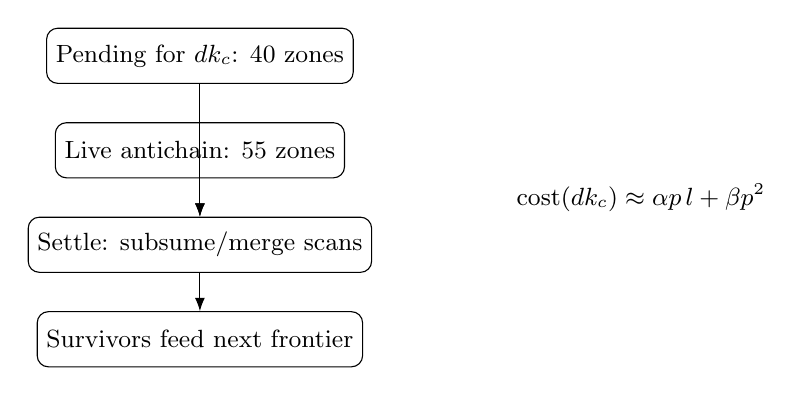
\begin{tikzpicture}[>=Latex, font=\small]
  \tikzstyle{box}=[draw, rounded corners, minimum width=33mm, minimum height=7mm]
  \node[box] (p0) at (0,0) {Pending for $dk_c$: 40 zones};
  \node[box] (l0) at (0,-1.2) {Live antichain: 55 zones};
  \node[box] (m0) at (0,-2.4) {Settle: subsume/merge scans};
  \node[box] (o0) at (0,-3.6) {Survivors feed next frontier};

  \draw[->] (p0) -- (m0);
  \draw[->] (l0) -- (m0);
  \draw[->] (m0) -- (o0);

  \node at (5.6,-1.8) {$\cost(dk_c) \approx \alpha p\,l + \beta p^2$};
\end{tikzpicture}
\caption{A heavy chain forms when both pending and live sets are large.}
\label{fig:chain-growth}
\end{figure}


\section{Load Imbalance Across Frontier Levels (Detailed)}
\subsection{Level-synchronous execution model}
Let level $L$ produce task set $\{\tau_i\}_{i=1}^{m_L}$, where each task is one chain settle for key $dk_i$.
With $P$ worker threads and a barrier at level end, level makespan is:
\[
T_L = \max_{p\in\{1,\dots,P\}} \sum_{\tau_i\in\mathcal{W}_p} C_i + B_L,
\]
where $C_i$ is chain cost and $B_L$ is barrier/synchronization overhead.

If costs are highly skewed, then $T_L$ is dominated by a small subset of chains.

\paragraph{Plain-language reading of the formula.}
At one frontier level, each thread gets a bag of chain tasks.
The level cannot finish until the \emph{slowest} thread finishes its bag.
So the term
\[
\max_p \sum_{\tau_i\in\mathcal{W}_p} C_i
\]
means ``the most overloaded thread decides the level time.''
The extra term $B_L$ is the fixed wait/synchronization cost paid by everyone at the end.

\paragraph{Why this matters.}
Even if 31 threads finish quickly, one thread with a very heavy chain still blocks progression to the next level.
This is exactly why high core count does not guarantee high speedup in level-synchronous symbolic search.

\subsection{Why successor fanout creates skew}
For a chain keyed by $dk$:
\[
C(dk) \approx c_1\,|\Pend_{dk}|\,|\Live_{dk}| + c_2\,|\Pend_{dk}|^2 + c_3\,M(dk),
\]
where:
\begin{itemize}
  \item $|\Pend_{dk}|$: new zones this level,
  \item $|\Live_{dk}|$: current antichain size,
  \item $M(dk)$: successful/attempted convex-union operations.
\end{itemize}
Uneven successor fanout makes $|\Pend_{dk}|$ heavy-tailed across keys.
If large fanout also lands on already-large antichains, cost becomes superlinear.

\paragraph{What ``uneven successor fanout'' means concretely.}
From one frontier level, each parent symbolic state generates a variable number of successors.
Those successors are then projected to keys $dk$.
If many parents happen to project to the \emph{same} key, that key's pending list explodes.
Other keys may receive only one or two pending zones.

\paragraph{Why this happens in timed symbolic models.}
This concentration is structural, not random noise:
\begin{itemize}
  \item synchronization patterns can funnel many transitions into the same discrete control state,
  \item zone abstraction merges many concrete valuations under identical discrete locations/integers,
  \item extrapolation/subsumption can keep some keys compact while others remain large and active.
\end{itemize}
So the algorithm naturally creates hot and cold keys at the same level.

\paragraph{Interpreting the proxy cost terms.}
\begin{itemize}
  \item $c_1|\Pend||\Live|$: each pending candidate is compared against many live survivors.
  \item $c_2|\Pend|^2$: pending candidates also interact indirectly through kill/merge effects.
  \item $c_3M(dk)$: successful/attempted convex unions add extra matrix work.
\end{itemize}
When both $|\Pend|$ and $|\Live|$ are large, this key becomes a straggler.

\subsection{Starvation (tail) condition}
Define total useful work in a level:
\[
W_L = \sum_{i=1}^{m_L} C_i,
\]
and ideal balanced time $W_L/P$.
A practical starvation indicator is:
\[

\paragraph{Interpretation of $\rho_L$.}
If $\rho_L=1$, the heaviest chain is about as large as ``fair share'' per worker.
If $\rho_L=4$, then one chain alone costs four workers' fair-share budget.
In that situation, no scheduling trick can fully hide the tail at that level; most workers will finish early and wait.

\paragraph{A concrete mini-scenario.}
Assume $P=8$ threads and total level work $W_L=800$ units, so ideal is $W_L/P=100$.
If one hot chain has $C_{max}=320$, then
\[
\rho_L = 320/100 = 3.2.
\]
That single chain already needs over three ideal worker budgets, so noticeable idle time is unavoidable unless the chain itself can be split.
\rho_L = \frac{\max_i C_i}{W_L/P}.
\]
When $\rho_L \gg 1$, one chain alone exceeds ideal per-thread budget and threads must idle near barrier.

\subsection{Observed effect in this checker}
The checker is level-synchronous; therefore tail chains directly delay the next level.
Even with dynamic scheduling, once only one or two heavy chains remain, available parallelism collapses.
This explains why adding threads can stop helping (or regress due to overhead).

\paragraph{Thread timeline intuition.}
At the start of a level, all workers are busy.
As light chains complete, workers become idle.
Near level end, only the hot chains remain, often on one or two workers.
The remaining workers wait at the barrier.
This ``long tail'' repeats every level where chain skew is high.

\paragraph{Key takeaway.}
The bottleneck is not ``insufficient thread count.''
The bottleneck is \emph{per-level skew in chain costs} under barrier synchronization.
So the primary optimization target is tail reduction: cost-aware ordering, heavy-chain chunking, and adaptive policy selection.

\begin{figure}[t]
\centering
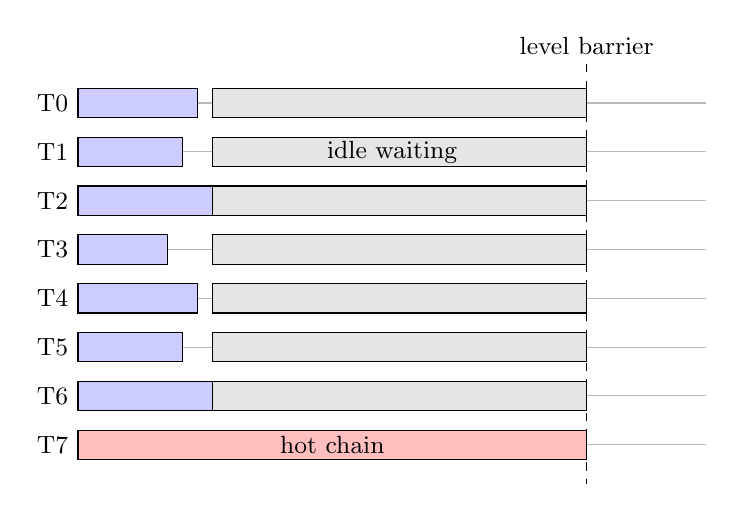
\begin{tikzpicture}[x=0.19cm,y=0.62cm,>=Latex, font=\small]
  \foreach \i/\lbl in {0/T0,1/T1,2/T2,3/T3,4/T4,5/T5,6/T6,7/T7} {
    \draw[gray!55] (0,-\i) -- (42,-\i);
    \node[left] at (0,-\i) {\lbl};
  }

  % light tasks
  \filldraw[draw=black,fill=blue!20] (0,-0.3) rectangle (8,0.3);
  \filldraw[draw=black,fill=blue!20] (0,-1.3) rectangle (7,-0.7);
  \filldraw[draw=black,fill=blue!20] (0,-2.3) rectangle (9,-1.7);
  \filldraw[draw=black,fill=blue!20] (0,-3.3) rectangle (6,-2.7);
  \filldraw[draw=black,fill=blue!20] (0,-4.3) rectangle (8,-3.7);
  \filldraw[draw=black,fill=blue!20] (0,-5.3) rectangle (7,-4.7);
  \filldraw[draw=black,fill=blue!20] (0,-6.3) rectangle (9,-5.7);

  % one heavy chain
  \filldraw[draw=black,fill=red!25] (0,-7.3) rectangle (34,-6.7);

  % idle tails
  \foreach \i in {0,1,2,3,4,5,6} {
    \filldraw[draw=black,fill=gray!20] (9,-\i-0.3) rectangle (34,-\i+0.3);
  }

  \draw[dashed] (34,0.8) -- (34,-7.8);
  \node[above] at (34,0.8) {level barrier};

  \node at (17,-7.0) {hot chain};
  \node at (21,-1.0) {idle waiting};
\end{tikzpicture}
\caption{Starvation/tail effect: one hot chain dominates level completion while other threads idle.}
\label{fig:parallel-starvation}
\end{figure}


\section{Related Approaches for Similar Irregular Tasks}
The same pattern appears in graph analytics, sparse linear algebra, SAT/SMT propagation, and symbolic model checking.
Common strategies:

\subsection*{1) Cost-aware scheduling}
Estimate $\hat C(dk)$ online and process heavy chains first.
This reduces end-of-level tails.

\subsection*{2) Work stealing with heavy-task splitting}
Idle workers steal remaining tasks.
For very large chains, split into bounded chunks and requeue, preserving local order constraints.

\subsection*{3) Hybrid policies}
Switch between incremental insertion and fused settle based on observed skew and contention.
No single policy is best across all levels.

\subsection*{4) Hierarchical queues}
Maintain separate heavy/light queues; keep heavy queue globally visible and light queue local to reduce contention.

\subsection*{5) NUMA-aware ownership}
Keep frequently-hit chains on stable worker sockets when possible, reducing remote memory penalties.

\section{Actionable Design for PTCTCL}
\subsection*{Step A: Instrument first}
Per level, emit:
\begin{itemize}
  \item touched chain count,
  \item pending-size distribution (median/p95/max),
  \item live-size distribution,
  \item top-k chain settle times,
  \item idle tail fraction near barrier.
\end{itemize}

\subsection*{Step B: Predictive ordering}
Build vector $V_L=\{(dk,\hat C)\}$ with
\[
\hat C = a\,|\Pend_{dk}|\,|\Live_{dk}| + b\,|\Pend_{dk}|^2,
\]
sort descending, schedule dynamically.

\subsection*{Step C: Heavy-chain chunking}
For chains with $|\Pend_{dk}| > \tau$, settle only $K$ pending entries, then requeue remainder.
This improves fairness and reduces tail without changing logical checks.

\subsection*{Step D: Adaptive policy}
At each level choose policy:
\begin{itemize}
  \item low skew: incremental path,
  \item high skew/high contention: fused path + predictive ordering + chunking.
\end{itemize}

\subsection*{Correctness note}
Any optimization must preserve the chain-local semantic constraints (subsumption and union behavior under accepted ordering rules).
Hence implementation should change scheduling granularity, not logical predicates.

\section{Conclusion}
The key bottleneck is not simply thread count; it is chain-level irregularity under level barriers.
A small number of hot chains can dominate per-level makespan, creating starvation of otherwise idle workers.

The right optimization objective is therefore tail reduction under semantic constraints:
measure skew, predict heavy chains, schedule by cost, and chunk heavy settles when needed.
These are established techniques in irregular parallel systems and are directly applicable here.


\end{document}
